\documentclass[10pt,twocolumn,letterpaper]{article}

\usepackage{cvpr}
\usepackage{times}
\usepackage{epsfig}
\usepackage{graphicx}
\usepackage{amsmath}
\usepackage{amssymb}
\usepackage{hyperref}

% Include other packages here, before hyperref.

% If you comment hyperref and then uncomment it, you should delete
% egpaper.aux before re-running latex.  (Or just hit 'q' on the first latex
% run, let it finish, and you should be clear).
%\usepackage[pagebackref=true,breaklinks=true,letterpaper=true,colorlinks,bookmarks=false]{hyperref}

\cvprfinalcopy % *** Uncomment this line for the final submission

\def\cvprPaperID{****} % *** Enter the CVPR Paper ID here
\def\httilde{\mbox{\tt\raisebox{-.5ex}{\symbol{126}}}}

% Pages are numbered in submission mode, and unnumbered in camera-ready
%\ifcvprfinal\pagestyle{empty}\fi
\setcounter{page}{1}
\begin{document}

%%%%%%%%% TITLE
\title{Social Network Using Image (SNUI)}

\author{
Anjan Nepal\\
Temple University\\
{\tt\small anjan.nepal@temple.edu}
% For a paper whose authors are all at the same institution,
% omit the following lines up until the closing ``}''.
% Additional authors and addresses can be added with ``\and'',
% just like the second author.
% To save space, use either the email address or home page, not both
\and
Qingqing Cai\\
Temple University\\
{\tt\small qingqing.cai@temple.edu}
}

\maketitle
%\thispagestyle{empty}

%%%%%%%%% ABSTRACT
\begin{abstract}
There is a rise in the number of social networking websites which facilitate in building of social relations among people who share similar interests and activities. Many of these websites allow people to upload and share images, but the content of the images is usually neglected. In this project, we develop a simple social networking site (SNUI) focusing mainly on the content in the pictures that are posted by the users. We want to provide the functionality of searching by image content, recommending friend suggestion based on the similar images they both have, and splitting the album grouping the images into different groups. Using features based on color correlogram, we show that the results are promising and this approach can open up a new way people use the social network websites.
\end{abstract}

%%%%%%%%% BODY TEXT
\section{Introduction}
Social network is an internet-based platform for communication, whose communication nodes are connected under the same or simiar network. Building a social network site helps people to be together for chatting, exchanging ideas or sharing feelings. Also, it changes traditional marketing channels, and benefits small business. For example, a social network enables salesmen to turn those likes and follows as customer engagement and increase sales. Moreover, it enables salesmen to further broad the market, since they can find new customers with similar interests.

The first social network site SixDegrees was launched in 1997, allowing users to create profiles, list their friends, and surf the friends list. And SixDegrees promoted itself as a tool to help people connect with and send messages to others. While SixDegrees attracted millions of users, it failed to become a sustainable business, and in 2000, the service closed. The next wave of Social Networks began when Ryze was launched in 2001 to help people leverage their business networks. At the same time, there are some other similar websites, such as Tribe.net, LinkedIn and Friendster. The people behind these websites were tightly entwined personally and professionally. But in the end, Ryze never acquired mass popularity, Tribe.net became a powerful business service and Friendster became the most significant. Nowadays, besides Friendster, there are some other popularly used social network websites, such as MySpace and Facebook.

Different from existing social network, our social network system supports image content based operations. As multi-media progresses nowadays, more and more users intend to upload photos they are interested in; also, users become more interested in broswing others' photos, instead of the status. However, current social network website do not support image retrieval. Making use of the image content and making applications based on that is a new and interesting path that the social networking websites should consider. 

To the best of our knowledge, there has been very few uses of the image content by the existing social networking websites. Picasa and Facebook use face-detection algorithm to find the faces of the people in the images for helping user to tag person. Flickr, a popular image uploading website does not make use the image contents. Google Image Search however allows users to search images based on the image content similarity, but it is not a social networking website and the applications of the image content are not used for the social network. In this project, we show that using image content can help improve the user experience in the social networking websites.
%-------------------------------------------------------------------------

\section{Approach}
In this project, we want to build a prototype application system which shows the potential of using the image content in the social networking websites. We mainly show how making use of the image content improves the user experience in the website. We do not build fully funtional website, which is out of the scope of what we try to show. In this section, we discuss the approaches we took to build the experimental application system.

\subsection{Functionality}
The following common type of functions could be handled by our target system.

\begin{itemize}
  \item \textbf{Registration}: 
  New users have to provide their personal information when they create an account, and our system will return a unique username and a password.
  \item \textbf{Upload}: 
  Users are allowed to upload photos into one of their albums. 
  \item \textbf{Browse Images}: 
  Users can browse the images in an album.
  \item \textbf{Friend request}: 
  Based on the image similarity with other user, the user can be suggested to send a friend request to the other user.
\end{itemize}

Besides these functionalities described above, our system also supports content based retrieval. Specifically, there are two actions. 

\begin{itemize}
  \item \textbf{Image searching and friend suggestion}: 
  Users can issue an image query, and all similar visible photos are returned, specifying which users these photos belong to. Based on the retrieval results, users can send the friend request to a person who may share the similar interests.
  \item \textbf{Image clustering}: 
  Split photos in one album into other (existing or new) albums according to the similarities among photos. For this, we used the K-means clustering. The user inputs the number of albums (K) in which the current set of photos can be divided and the images will be grouped into these clusters based on their similarities.
\end{itemize}

\subsection{Database Design}
In this application, we have focused mainly on the image content based retrieval and most of the work has been focused in developing the application for such. In this section we discuss the database design that we considered.
\subsubsection{Schema}
We firstly built a relational model as follows:
\begin{itemize}
	\item User (\emph{\underline{userID}}, \emph{username}, \emph{password}, \emph{firstName}, \emph{lastName}, \emph{address}, \emph{birthday}, \emph{gender}, \emph{isActive}, \emph{imagePath})

	\item Photo (\emph{\underline{photoID}}, \emph{albumID}, \emph{caption}, \emph{featureValue}, \emph{locationPath}, \emph{thumnailPath}, \emph{isRGB}, \emph{uploadTime})

	\item Album (\emph{\underline{albumID}}, \emph{userID}, \emph{thumnailPhotoID}, \emph{albumName}, \emph{description}, \emph{visibility})

	\item photoLike (\emph{\underline{userID}}, \emph{\underline{photoID}}, \emph{dataTime}, \emph{isNotified})

	\item friendRequest (\emph{\underline{senderID}}, \emph{\underline{receiverID}}, \emph{\underline{dateTime}}, \emph{isNotified})

	\item friendship (\emph{\underline{userID1}}, \emph{\underline{userID2}}, \emph{startDateTime}, \emph{isNotified})

	\item comment (\emph{\underline{commentID}}, \emph{commenterID}, \emph{photoID}, \emph{text}, \emph{dateTime}, \emph{isNotified})
\end{itemize}

Details for each table are described as follows.

\begin{enumerate}
  \item In User, we record each user's personal information, such as userID, username, password, firstName, etc. A unique userID is to identify a distinct user; userName and password are needed to access the online database.
  \item For each photo, we need to specify which album it belongs to by checking albumID; the photo informationm, such as caption, isRGB, is useful for image retrieval in our furture design. For storing the features, a double vector is used as the attribute type.
  \item Album is a collection of photos, and it beongs to a particular user. A privacy setting is applied in our system, retricting the visibility of the album posted on the site. It has three possible values PRIVATE, FRIENDS, EVERYONE.
  \item PhotoLike is a relation connecting a user and photos they like. isNotified is TRUE when a user ``likes" the photo, and then the system sends a notification to the user who owns the photo. Comment supports users to comment photos posted online, and our system records the content and the post time. Also, notification is sent to the photo owner when the event is active.
  \item friendRequest is a request sending from userID1 to userID2. Once userID2 accepts the request, they become friends, and a new tuple is inserted in friendship. Notification is sent to corresponding users if necessary.
\end{enumerate}


%-------------------------------------------------------------------------
\section{Correlogram Feature}
The feature we used for image processing is color correlogram, which captures the spatial correlation of colors and describes the global distribution of local spatial correlation of colors. The correlogram robustly tolerates large changes in appearance and shape caused by changes in viewing positions, camera zooms, etc. And the size of the feature is fairly small.

Informally, a color histogram of an image is a table indexed by color pairs, where the $k$-th entry for $<i,j>$ specifies the probability of finding a pixel of color $j$ at a distance $k$ from a pixel of color $i$ in the image. To define the correlogram mathematically, let $I$ be an $n \times n$ image. The colors in $I$ are quantized into $m$ colors $c_{i},\ldots,c_{m}$. A distance $d \in [n]$ be fixed as a priori. Then, the correlogram of $I$ is defined as:
\begin{equation}
	\begin{aligned}
		\gamma_{c_{i},c_{j}}^{(k)} \triangleq Pr_{p_{1} \in I_{c_{i}},p_{2} \in I} [p_{2} \in I_{c_{j}}||p_{1}-p_{2}|=k].
	\end{aligned}
\end{equation}
Given any pixel of color $c_{i}$ in the image, $\gamma_{c_{i},c_{j}}^{(k)}$ gives the probability that a pixel at distance $k$ away from the given pixel is of color $c_{j}$.

Based on the correlogram definition, the autocorrelogram of $I$ captures spatial correlation between identical colors only and is defined by:
\begin{equation}
	\begin{aligned}
		\alpha_{c}^{(k)}(I) \triangleq \gamma_{c,c}^{(k)}(I)
	\end{aligned}
\end{equation}
This information is a subset of the correlogram and requires only $O(md)$ space, while the size of correlogram is $O(m^2d)$.
In our project, only 256 different colors are used for one image, and the initial distance vector is $[1,3,5,7]$, so the feature size is 1024.

The image searching problem is defined as: let $D$ be an image database and $Q$ be the query image, assign $rank(I) \in [|D|]$ for each $I \in D$, using some notion of similarity to $Q$. The $L_{1}$ distance is a commonly used similarity measurement when comparing two feature vectors. And the $L_{1}$ is defined as:
\begin{equation}
	\begin{aligned}
		|I-I'|_{\gamma,L_{1}} \triangleq \sum_{i,j \in [m],k \in [d]} |\gamma_{c_{i},c_{j}}^{(k)}(I)-\gamma_{c_{i},c_{j}}^{(k)}(I')|
	\end{aligned}
\end{equation}

%-------------------------------------------------------------------------
\section{Implementation Details}
In this section, we present implementation details in designing our system SNUI. The details cover Registration, Photo uploading and View, Image Searching and Clustering. We have build the application so that it is robust to various factors like errors, failure in form validation, malicious user attempts, lack of atomicity etc. We discuss them in details below.

We have implemented security and correctness in our program. A user can only perform actions that he is allowed to do. For this, the user information is saved in the session variable and checked if the session information and the action being done matches. If not, then the action is not performed. For example, if a user tries to upload a photo to an album belonging to a different user, then the action is not performed.

A user can log in if he has an account in SNUI, otherwise, he needs to provide required information and register for a new account. If the user does not type required fields, he is redirected to the form. If the username has already been taken, then he is asked to provide a different username. A registered user can login after providing the username and password that matches. He can perform several actions and can logout to clear the session.

Whenever a user uploads a photo, the real-time correlogram feature is computed and stored in the database as a double array. We do not actually save the image content in the database but only store the image url in the database and store the actual file in the filesystem. Since the image name saved in the filesystem could have conflicts, the next photo id is asked from the database ( eg. nextval() in Postgres ). Then, this id is used to save the file to the filesystem and also to the database. This also ensures that the atomicity of the image upload is saved.

For image searching, when the user issues an image query, the correlogram feature is computed and compared with those feature vectors extracted from our database. The results are ranked according to the L1 distance between two feature vectors. To get the owner of an image, we do the join among ``User", ``Album" and ``Photo" by using the SQL statement as follows:

\emph{\textbf{select} User.userID}\newline \indent
\emph{\textbf{from} Photo,Album,User}\newline \indent
\emph{\textbf{where} Photo.albumID=Album.albumID}\newline \indent \indent \indent
\emph{\textbf{and} Album.userID=User.userID}

In image clustering, users are required to specify $k$, the number of splits to make. From the album, we randomly select $k$ images and set them as the initial groups. Then, assign each object to the group that has the closest centroid, and recalculate the new controid for each group; The previous two steps are repeated until the centroids no longer move.

%-------------------------------------------------------------------------
\section{Software and Tools}
The database system we used is PostgreSQL\cite{postgres}. It implements the majority of the SQL:2008 standard, is ACID-compliant, is fully transactional (including all DDL statements), has extensible data types, operators, index methods, functions, aggregates, procedural languages, and has a large number of extensions written by third parties. We used the PostgreSQL that was installed with the Linux distro Ubuntu, which we used for the development. For the web application part, we used PHP\cite{php}. PHP is used for developing dynamic and interactive web pages. It is one of the first developed server-side scripting languages to be embedded into an HTML source document rather than calling an external file to process data. The code is interpreted by a Web server with a PHP processor module which generates the resulting Web page. We used Apache\cite{apache} as our web server. Git\cite{git} was used for the concurrency version control. To compute correlogram features, we used a Java Package LIRE (Lucene Image REtrieval) library.

%-------------------------------------------------------------------------
\section{Demo/Manual}
This section presents a brief demo of the application showing how to use it. It is also available online at \url{http://ec2-184-73-14-96.compute-1.amazonaws.com/sn/}.

The registration page is shown in figure \ref{fig:registration}.

\begin{figure}[t]
\begin{center}
\fbox{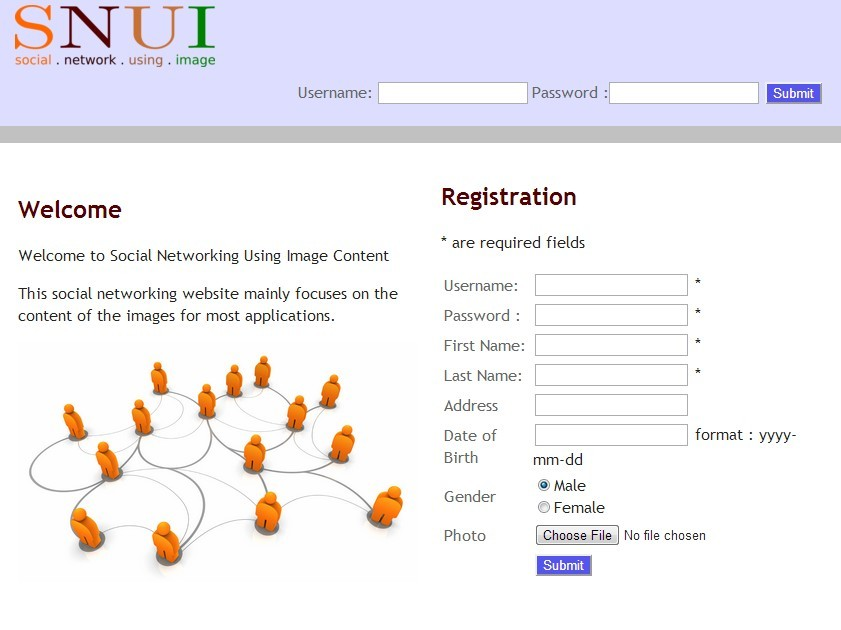
\includegraphics[height=5cm,width=8cm]{registration.jpg}}
\end{center}
\caption{Registration Page of SNUI}
\label{fig:registration}
\end{figure}

A member could log in if he has an account in our system, but new users should register and provide some required information firstly.

After logging in, users have some optional operations, such as ``View Albums", ``Create new album", ``Add photos", ``Search photos" and ``Logout", as shown in figure ~\ref{fig:operations}.

\begin{figure}[t]
\begin{center}
   \fbox{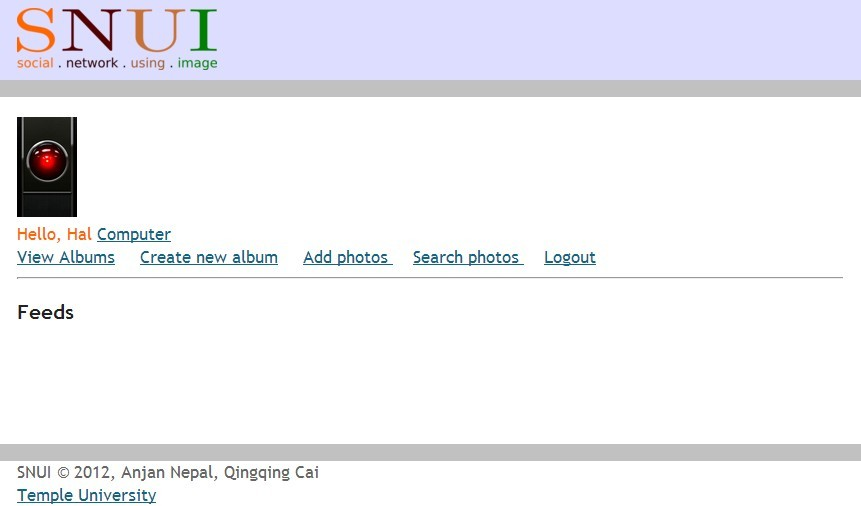
\includegraphics[height=5cm,width=8cm]{profile.jpg}}
\end{center}
\caption{Possible Operations Provided in SNUI}
\label{fig:operations}
\end{figure}

To create a new album, the user needs to provide the album name, and give the description. A privacy setting is applied in our system, restricting the visibility of the album posted on the site to be ``private", ``friends" or ``everyone" (figure ~\ref{fig:album}). Before adding a photo, we need to specify which album this photo belongs to, either choosing an existing album or creating a new album (figure ~\ref{fig:addphoto}).

\begin{figure}[t]
\begin{center}
  \fbox{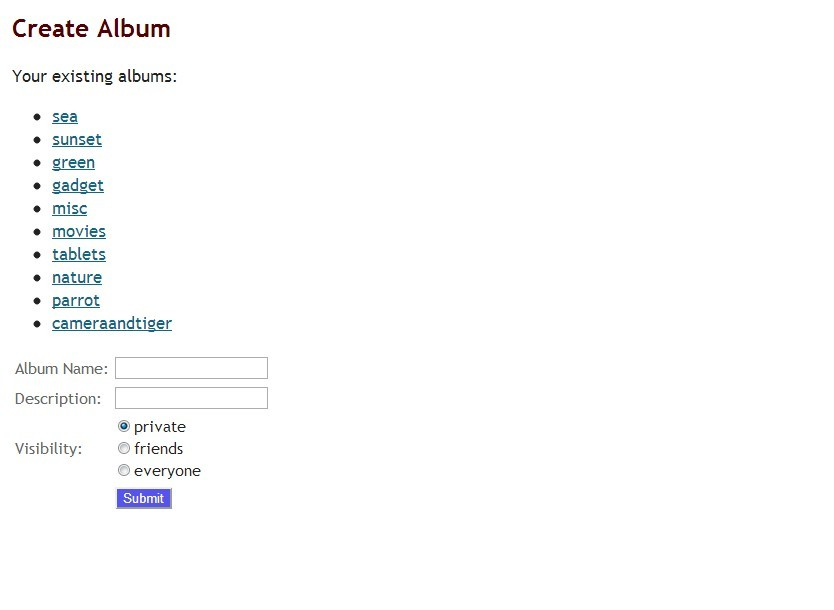
\includegraphics[height=5cm,width=8cm]{createnewalbum.jpg}}
\end{center}
\caption{Description in Creating New Albums}
\label{fig:album}
\end{figure}

\begin{figure}[t]
\begin{center}
   \fbox{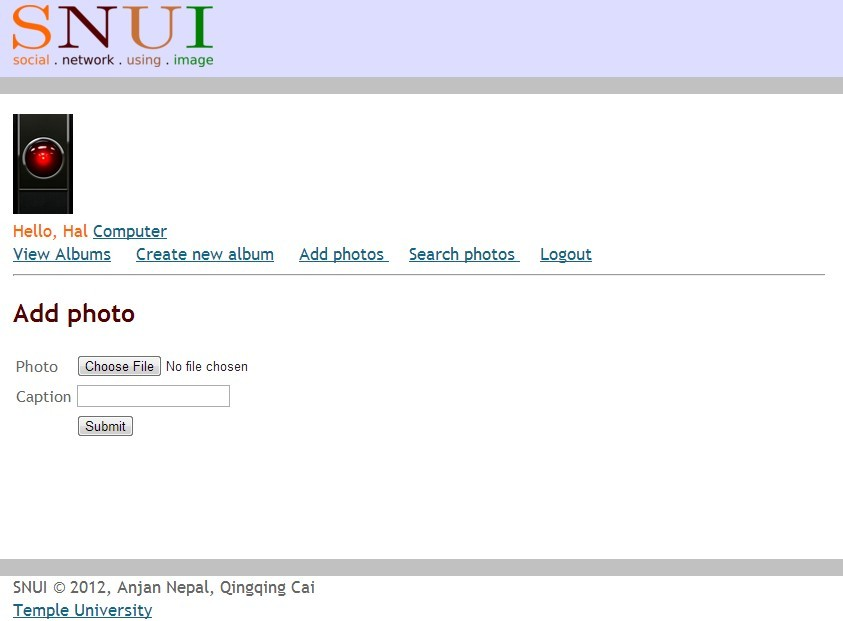
\includegraphics[height=5cm,width=8cm]{addphotos.jpg}}
\end{center}
\caption{Description in Adding Photos}
\label{fig:addphoto}
\end{figure}

Photos in an album can be splited into $k$ sub-groups, by clicking ``Cluster Album" under ``View Album". After specifying the number $k$, we can name the sub-group, and generate a new album, shown in figure ~\ref{fig:split}.

\begin{figure}[t]
\begin{center}
\fbox{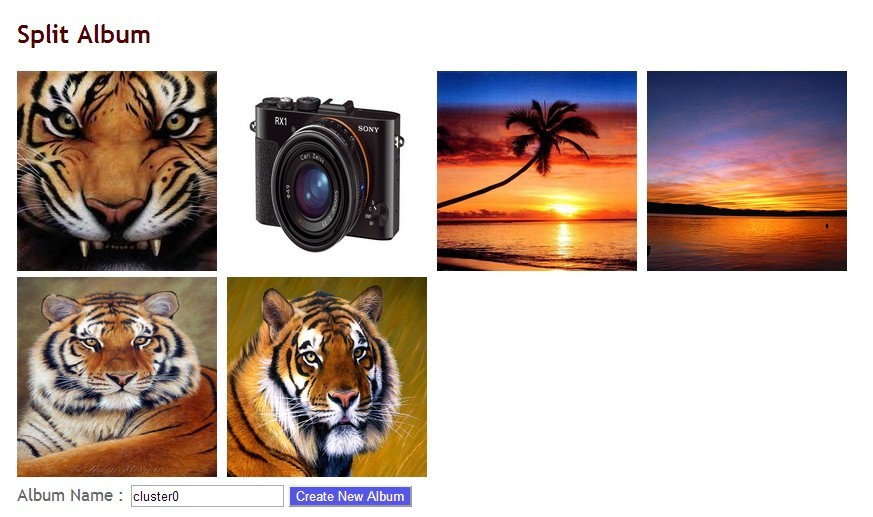
\includegraphics[height=5cm,width=8cm]{splitalbum.jpg}}
\end{center}
\caption{Example for Album Spliting}
\label{fig:split}
\end{figure}

The photo searching part is shown in figure ~\ref{fig:suggestion}. After issuing an image query, the feature is computed and compared with all candidates in our dataset, and results are ranked according to the $L_1$-norm distance between two feature vectors. In addition, our system shows which user the result image belongs to. If the retrieved image is neither the user himself nor the user's friend, then a friend request could be sent from the current user to the image owner.

\begin{figure}[t]
\begin{center}
\fbox{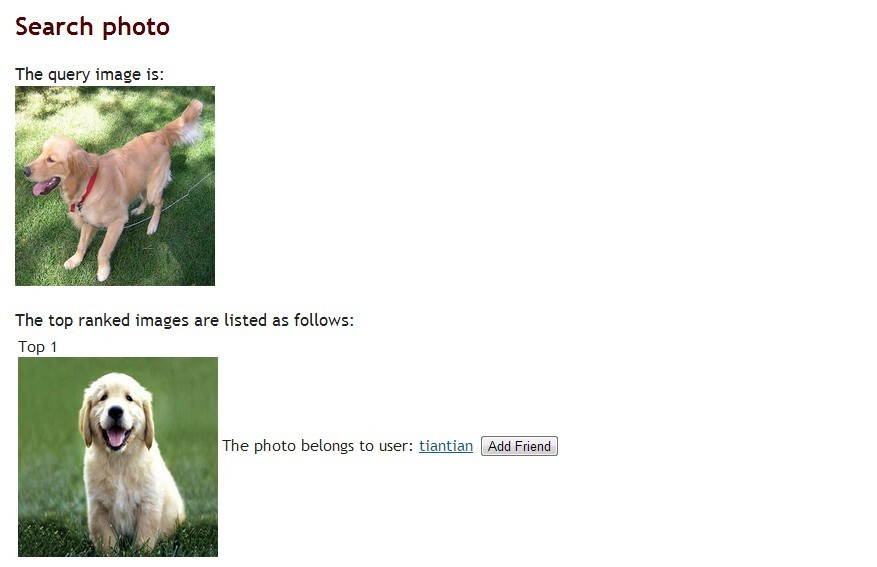
\includegraphics[height=5cm,width=8cm]{searchphoto.jpg}}
\end{center}
\caption{Example for Photo Searching and Friend Suggestion}
\label{fig:suggestion}
\end{figure}

%-------------------------------------------------------------------------
\section{Discussion and Future Directions}
In this project, we provided and designed a Social Network Using Images (SNUI), which is a simple social network mainly focusing on the content of images uploaded online. The objective of SNUI is to support image searching and clustering, and to support friends recommendation based on the similar images they both have. The image feature we used in our project is color correlogram, capturing and describing the distribution the spatial correlation of colors. As future work, we need to improve the image processing by using more features which can consider other image content information. Some of these can be texture features, shape features etc. Also, the surrounding text and the caption of photos can also be used to increase the accuracy of the image content based operations. The image search based on similarity requires a comparison between a lot of images in the database. For the scalability, the similarity between the images can be precomputed and stored in the database for the faster retrieval.

%-------------------------------------------------------------------------
\begin{thebibliography}{50}
 \bibitem{correlogram} Huang, Jing, et al. ``Image indexing using color correlograms." Computer Vision and Pattern Recognition, 1997. Proceedings., 1997 IEEE Computer Society Conference on. IEEE, 1997.
 \bibitem{git} \url{http://git-scm.com/}
 \bibitem{postgres} \url{http://www.postgresql.org/}
 \bibitem{php} \url{http://www.php.net/}
 \bibitem{apache} \url{http://www.apache.org/}
\end{thebibliography}

\end{document} 
